\part{Testcontent}
\chapter{Allgemeine Sachen}
abcdefghijklmnopqrstuvwxyz \\
ABCDEFGHIJKLMNOPQRSTUVWXYZ \\
1234567890!?.:,;

\section{Mathezeug}
\begin{math}
abcdefghijklmnopqrstuvwxyz\\
ABCDEFGHIJKLMNOPQRSTUVWXYZ\\
\mathbb{ABCDEFGHIJKLMNOPQRSTUVWXYZ}\\
\mathscr{ABCDEFGHIJKLMNOPQRSTUVWXYZ}\\
1234567890 + - \times \div\\
\int \iint \iiint \oiint \oiiint
\end{math}
\subsection{Eingerückte Formeln}
\[\frac{1}{2 \pi i} \int_{\gamma} f = \sum_{k = 1}^{m} n (\gamma; a_k)\text{Res}(f; a_k)\]
\[\mathbf{B}(P)=\frac{\mu_0}{4\pi}\int\frac{\mathbf{I}\times\hat{r}'}{r'^2}dl = \frac{\mu_0}{4\pi}\int\frac{d\mathbf{l}\times\hat{r}'}{r'^2}dl\]
\[\sum_{x = 0}^{100} x + x\]
\subsection{Gleichungen}
\begin{align*}
	L & = \lim_{|x| \to \infty}\ \frac{\cos \frac 1x \cdot \frac{-1}{x^2}}{\frac{-1}{x^2}}\\
	& = \lim_{|x| \to \infty} {\cos\frac 1x} \cdot \frac{-1}{x^2} \cdot \frac{x^2}{-1}\\
	& = \cos\frac 1{\infty} = \cos 0 = 1
\end{align*}

\subsection{Text in Matheumgebungen}
$\sum_{\text{Von Null}}^{\text{bis zur Unendlichkeit}} x \text{ text passt die gre der Schrift Automatisch an.}$

$\sum_{\mbox{Von Null}}^{\mbox{bis zur Unendlichkeit}} x \mbox{ mbox nimmt immer die normale gre der schrift.}$

\section{Pakettests}
Dies ist ein Kurzer Test um ein \ac{acr} zu verdeutlichen wie man sehen kann wird nur beim ersten benutzen des ''ac'' Befehls das \ac{acr} voll ausgeschrieben.\\
Normales ref\index{ref!Normales}: \ref{EndeDesTextes}\\
Verbessertes ref:\index{ref!Verbessertes} \vref{EndeDesTextes}\\
Verweis auf Literaturverzeichnis mit BiBTex (siehe \cite{wiki:Latex}): Blablabla sagte Wikipedia \cite{wiki:LatexTwo}.

\section{Enumerate}
\begin{enumerate}
\item Test 1
\item Test 2
\item Test 3
		\begin{enumerate}
		\item Test 3.1
		\item Test 3.2
		\item Test 3.3
				\begin{enumerate}
				\item Test 3.3.1
				\item Test 3.3.2
				\item Test 3.3.3
				\end{enumerate}
		\end{enumerate}
\end{enumerate}

\subsection{abc Enumerate}
\begin{enumerate}[label=\alph*)]
\item Test 1
\item Test 2
\item Test 3
		\begin{enumerate}[label=\arabic*)]
		\item Test 3.1
		\item Test 3.2
		\item Test 3.3
				\begin{enumerate}[label=\Roman*)]
				\item Test 3.3.1
				\item Test 3.3.2
				\item Test 3.3.3
				\end{enumerate}
		\end{enumerate}
\end{enumerate}

\section{Itemize}
\begin{itemize}
\item Test 1
\item Test 2
\item Test 3
		\begin{itemize}
		\item Test 3.1
		\item Test 3.2
		\item Test 3.3
				\begin{itemize}
				\item Test 3.1
				\item Test 3.2
				\item Test 3.3
				\end{itemize}
		\end{itemize}
\end{itemize}

\subsection{arrow Itemize}
\begin{itemize}[label=$\rightarrow$]
\item Test 1
\item Test 2
\item Test 3
		\begin{itemize}
		\item Test 3.1
		\item Test 3.2
		\item Test 3.3
		\end{itemize}
\end{itemize}

\section{Script Test}
\subsection{Abk�rzungen}
$\sinx{90}$\\
$\cosx{90}$\\
$\tanx{90}$\\
$\dimx{90}$\\
$\spanx{90}$

\subsection{Hervorgehobene Indexe}
\indexn{Test Normal}, \indexn[Test Normal!Test Normal Sub]{Test Normal Sub}\\
\indexu{Test Underlined}, \indexu[Test Underlined!Test Underlined Sub]{Test Underlined Sub}\\
\indexi{Test Italic}, \indexi[Test Italic!Test Italic Sub]{Test Italic Sub}\\
\indexb{Test Bold}, \indexb[Test Bold!Test Bold Sub]{Test Bold Sub}\\

\subsection{R�mische Zahlen}
\RM{1}, \RM{2}, \RM{3}\\
\RM{1768}, \RM{126}

\subsection{Beispiel}
\bsp[Zusatztext]{Beispiel:}{
Die ist ein kurzes Beispiel um zu demonstrieren wie schn das hier eingerckt wird.

\begin{itemize}[label=\hra]
\item Test 1
\item Test 2
\item Test 3
		\begin{itemize}[label=\Ra]
		\item Test 3.1
		\item Test 3.2
		\item Test 3.3
		\end{itemize}
\end{itemize}

\lipsum[1]
\[\phi_n(\kappa) = \frac{1}{4\pi^2\kappa^2} \int_0^\infty
\frac{\sin(\kappa R)}{\kappa R} \frac{\partial}{\partial R}
\left[ R^2 \frac{\partial D_n(R)}{\partial R} \right]\mathrm dR\]
\lipsum[2-3]

\begin{enumerate}[label=zu \alph*)]
\item Test 1
\item Test 2
\item Test 3
		\begin{enumerate}[label=\arabic*)]
		\item Test 3.1
		\item Test 3.2
		\item Test 3.3
				\begin{enumerate}[label=\Roman*)]
				\item Test 3.3.1
				\item Test 3.3.2
				\item Test 3.3.3
				\end{enumerate}
		\end{enumerate}
\end{enumerate}

\lipsum[4]

\begin{enumerate}
\item Test 1
\item Test 2
\item Test 3
		\begin{enumerate}
		\item Test 3.1
		\item Test 3.2
		\item Test 3.3
				\begin{enumerate}
				\item Test 3.3.1
				\item Test 3.3.2
				\item Test 3.3.3
				\end{enumerate}
		\end{enumerate}
\end{enumerate}
}

\section{Lipsum}
\lipsum

\lipsum

\lipsum

\lipsum

\part{part}
\chapter{chapter}
\section{section}
\subsection{subsection}
\subsubsection{subsubsection}
\paragraph{paragraph}

\part{\texorpdfstring{$mathpart$}{mathpart}}
\chapter{\texorpdfstring{$mathchapter$}{mathchapter}}
\section{\texorpdfstring{$mathsection$}{mathsection}}
\subsection{\texorpdfstring{$mathsubsection$}{mathsubsection}}
\subsubsection{\texorpdfstring{$mathsubsubsection$}{mathsubsubsection}}
\paragraph{\texorpdfstring{$mathparagraph$}{mathparagraph}}

\label{EndeDesTextes}

\part{Beispiel}
\chapter{Elementare Rechenregeln}
\section{Zahlen}
\subsection{Natrliche, ganze und rationale Zahlen}
\subsubsection{Definitionsbereiche und Bezeichnungen}
Alle ganzen und gebrochenen Zahlen, die positiven und negativen sowie die Null, werden \indexi{rationale Zahlen} genannt. Man verwendet die folgenden Bezeichnungen.
\begin{itemize}
	\item Menge der natrlichen Zahlen: $\mb{N} = \gklamm{0, 1, 2, 3, \dots}$
	\item Menge der ganzen Zahlen: $\mb{Z} = \gklamm{\dots, -2, -1, 0, 1, 2, \dots}$
	\item Menge der rationalen Zahlen: $\mb{Q} = \gklamm{x \vert x = \frac{p}{q} \text{ mit } p \in \mb{Z}, q \in \mb{Z} \text{ und } q \neq 0}$
\end{itemize}
Die natrlichen Zahlen sind aus dem Bedrfnis des Abzhlens \ac{bzw.} des Ordnens entstanden. Die natrlichen Zahlen werden auch als \indexi{nichtnegative ganze Zahlen} bezeichnet.

\subsubsection{Eigenschaften der Menge der rationalen Zahlen}
\begin{itemize}
\item Die Menge der rationalen Zahlen ist unendlich.
\item Die menge ist \indexi{geordnet}, \ac{d.h.} fr je zwei verschiedene rationale Zahlen $a$ und $b$ kann man angeben, welche von beiden kleiner als die andere ist.
\item Die Menge ist \indexi{berall dicht}, \ac{d.h.}, zwischen je zwei verschiedenen rationalen Zahlen $a$ und $b$ ($a < b$) existiert wenigstens eine rationale Zahl $c$ ($a < c < b$). Daraus folgt, dass zwischen zwei verschiedenen rationalen Zahlen unendlich viele weitere rationale Zahlen liegen.
\end{itemize}

\subsubsection{Arithmetische Operationen}
Die arithmetischen Operationen (Addition, Subtraktion, Multiplikation, Division) mit zwei beliebigen rationalen Zahlen sind stets mglich und liefern im Ergebnis wieder eine rationale Zahl. Eine Ausnahme davon ist die \indexi{Division durch Null}, die \textit{unmglich} ist: Die Schreibweise $a : 0$ hat keinen bestimmten Sinn, da es keine bestimmte rationale Zahl $b$ gibt, die der Gleichung $b \mal 0 = a$ mit $a \neq 0$ gengt. Fr $a = 0$ kann $b$ eine beliebige rationale Zahl sein. Die oft verwendete Schreibweise $a : 0 = \infty$ (unendlich) bedeutet nicht, dass diese Division mglich ist; es ist lediglich eine Abkrzung fr die Aussage: Wenn sich der Nenner Null nhert, wchst der Quotient absolut genommen ber alle Grenzen.

\subsubsection{Dezimalbruch und Kettenbruch}
Jede rationale Zahl $a$ kann in der Form eines endlichen oder unendlichen periodischen Dezimalbruches oder auch in der Form eines Kettenbruches dargestellt werden.

\subsubsection{Geometrische Darstellung}
Wenn auf einer Geraden ein Anfangspunkt $0$ (\indexi{Nullpunkt}), eine positive Richtung (\indexi{Orientierung}) und eine Lngeneinheit $l$ (\indexi{Mastab}) festgelegt worden sind (\ac{Abb.} \vref{fig:Arithmetik_Zahlengerade}), dann entspricht jeder rationalen Zahl $a$ ein bestimmter Punkt dieser Geraden. Er hat die Koordinate $a$ und ist ein sogenannter \indexi{rationaler Punkt}. Die Gerade wird \indexi{Zahlengerade} genannt. Da die Menge der rationalen Zahlen berall dicht ist, gibt es zwischen je zwei beliebigen rationalen Punkten unendlich viele weitere rationale Punkte.
\begin{figure}[htb]
	\centering
	\captionsetup{labelformat=simple}
	\centering
	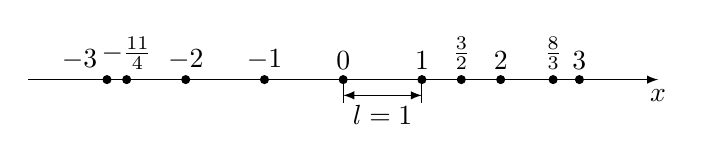
\begin{tikzpicture}
		\draw[-latex] (-4,0) -- (0,0) -- (4,0) node[below] {$x$};
		\foreach \x in {-2,-1,...,3}
			\draw[fill=black] (\x,0) circle (0.05) node[above] {$\x$};

		\draw[fill=black] (-3,0) circle (0.05) node[anchor=south east] {$-3$};
		\draw[fill=black] (-2.75,0) circle (0.05) node[above] {$-\frac{11}{4}$};
		\draw[fill=black] (1.5,0) circle (0.05) node[above] {$\frac{3}{2}$};
		\draw[fill=black] (2.666,0) circle (0.05) node[above] {$\frac{8}{3}$};

		\draw[latex-latex] (0,-0.2) -- (1,-0.2) node[midway, below] {$l = 1$};
		\draw (0,0) -- (0,-0.3);
		\draw (1,0) -- (1,-0.3);
	\end{tikzpicture}
	\caption{}
	\label{fig:Arithmetik_Zahlengerade}
\end{figure}

\subsection{Irrationale und transzendente Zahlen}
Fr die Analysis reicht die Menge der rationalen Zahlen nicht aus. Obgleich sie berall dicht ist, fllt sie nicht die gesamte Zahlengerade aus. Wenn man \ac{z.B.} die Diagonale $AB$ des Einheitsquadrats um $A$ dreht, so dass $B$in den Punkten $K$ der Zahlengraden bergeht (\ac{Abb.} \vref{fig:Arithmetik_DrehenDesEinheitsquadrates}), dann hat $K$ keine rationale Koordinate. Erst die Einfhrung der \indexi{irrationalen Zahlen} ermglicht es, jedem Punkt der Zahlengeraden eine Zahl zuzuordnen. Eine exakte Definition der irrationalen Zahlen kann \ac{z.B.} durch Intervallschachtelungen erfolgen oder mit Hilfe des \textsc{Dedekind}schen Schnittes. Fr die Anschauung gengt die Feststellung, dass die irrationalen Zahlen auf der Zahlengeraden die Punkte einnehmen, die als Lcke zwischen den rationalen Zahlen vorhanden sind, und dass jede irrationale Zahl durch einen nichtperiodischen unendlichen Dezimalbruch oder einen nichtperiodischen unendlichen Kettenbruch dargestellt werden kann.\\
\begin{figure}[htb]
	\centering
	\captionsetup{labelformat=simple}
	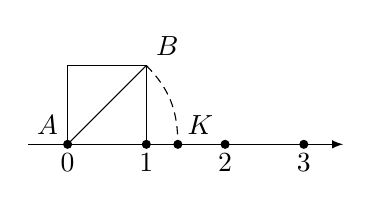
\begin{tikzpicture}
		\draw[-latex] (-0.5,0) -- (3.5,0);
		\foreach \x in {0,1,...,3}
			\draw[fill=black] (\x,0) circle (0.05) node[below] {$\x$};

		\draw[fill=black] (1.4,0) circle (0.05) node[anchor=south west] {$K$};

		\draw (0,0) rectangle (1,1);
		\draw (0,0) node[anchor=south east] {$A$} -- (1,1) node[anchor=south west] {$B$};

		\draw[densely dashed] (1,1) to [out=-45,in=90] (1.4,0);
	\end{tikzpicture}
	\caption{}
	\label{fig:Arithmetik_DrehenDesEinheitsquadrates}
\end{figure}
Zu den irrationalen Zahlen gehren insbesondere die nicht ganzzahligen reellen Wurzeln der algebraischen Gleichungen der Form
\begin{equation}
    x^n + a_{n - 1} x^{n - 1} + \dots + a_1 x + a_0 = 0 (n > 1, \text{ ganzzahlig; ganzzahlige Koeffizienten})\text{.}
\end{equation}
Man nennt solche Wurzeln \indexi{algebraische Irrationalitten}.
\begin{enumerate}[label=$\blacksquare$ \textbf{\Alph*:}, align=left, leftmargin=*]
\item Einfachste Beispiele fr algebraische Irrationalitten sind die reellen Wurzeln der Gleichungen $x^n - a = 0$, also Zahlen der Form $\sqrt[n]{a}$, wenn sie nicht rational sind.
\item $\sqrt[2]{2} = 1,414\dots$, $\sqrt[3]{10} = 2,154\dots$ sind algebraische Irrationalitten.
\end{enumerate}
\begin{enumerate}[label=$\blacksquare$ \textbf{\Alph*:}, align=left, leftmargin=*]
\item $\pi = 3,14592\dots$, $e = 2,718281\dots$ sind transzendente Zahlen
\item Die dekadischen Logarithmen der ganzen positiven Zahlen mit Ausnahme von Zahlen der Form $10^n$ sind transzendente Zahlen.\\
		Die nichtganzzahligen Wurzeln der quadratischen Gleichung
		\begin{equation}
			x^2 + a_1 x + a_0 = 0 (a_1, a_0 \text{ ganzzahlig})
		\end{equation}
		werden \indexi{quadratische Irrationalitten} genannt. Sie haben die Form $(a + b \sqrt{D}) \div c$ ($a, b, c$ ganzrational, $c \neq 0; D > 0$, quadratfrei).
\end{enumerate}
\begin{enumerate}[label=$\blacksquare$, align=left, leftmargin=*]
\item Die Teilung einer Strecke $a$ im Verhltnis des Goldenen Schnittes $x \div a = (a - x) \div x$ fhrt im Falle $a = 1$ auf die quadratische Gleichung $x^2 + x - 1 = 0$. Die Lsung $x = \left(\sqrt{5} - 1\right) \div 2$ ist eine quadratische Irrationalitt. Sie enthlt die irrationale Zahl $\sqrt{5}$.
\end{enumerate}

\subsection{Reelle Zahlen}
Alle rationalen und irrationalen Zahlen werden zu den reellen Zahlen zusammengefasst. Sie bilden die \indexi{Menge der reellen Zahlen}, die mit \mb{R} bezeichnet wird.
\subsubsection{Haupteigenschaften}
Die reellen zahlen besitzen die folgenden Haupteigenschaften:
\begin{itemize}
\item Die Menge der reellen Zahlen ist unendlich.
\item Die Menge der reellen Zahlen ist \indexi{geordnet}.
\item Die Menge der reellen Zahlen ist \indexi{berall dicht}.
\item Die Menge der reellen Zahlen ist \indexi{stetig}, \ac{d.h.}, jedem Punkt der Zahlengeraden entspricht eine reelle Zahl. Das gilt fr die Menge der rationalen Zahlen nicht.
\end{itemize}

\subsubsection{Arithmetische Operationen}
Die arithmetischen Operationen sind mit reellen Zahlen stets durchfhrbar und ergeben stets wieder eine reelle Zahl. Eine Ausnahme ist die Division durch Null. Das Potenzierten und seine Umkehrung sind ebenfalls im System der reellen Zahlen mglich; aus jeder positiven reellen Zahl lassen sich beliebige Wurzeln ziehen; zu jeder positiven reellen Zahl gibt es einen Logarithmus mit beliebiger positiven Basis, ausgenommen die Eins als Basis.\\
Eine weitergehende Verallgemeinerung des Zahlenbegriffs ist in der Analysis fhrt zu den \indexi{komplexen Zahlen}.

\subsubsection{Zahlenintervall}
Eine zusammenhngende Menge reeller Zahlen mit den Endpunkten $a$ und $b$, wobei $a < b$ ist und auch $a$ gleich $-\infty$ und $b$ gleich $+\infty$ sein kann, wird \indexi{Zahlenintervall mit den Endpunkten $a$ und $b$} genannt.\\
Wenn der Endpunkt nicht selbst zum INtervall gehrt, spricht man vom \indexi[offenes Intervallende]{offenen Intervallende}, im entgegengesetztem Falle vom \indexi[abgeschlossenes Intervall]{abgeschlossenen Intervallende}.\\
Die Angabe eines Zahlenintervalls erfolgt durch seine Endpunkte $a$ und $b$, indem diese in Klammern gesetzt werden. Eine eckige Klammer steht fr ein geschlossenes Intervallende, eine runde fr ein offenes. Es wird zwischen beiseits \indexi[beidseits offenes Intervall]{offenen Intervallen} $(a, b)$, \indexi[halboffenes Intervall]{halboffenen Intervallen} $\left[a, b\right)$ \ac{bzw.} $\left(a, b\right]$ und so weiter
